lllllllllllllllllllllllllllll%%%%%%%%%%%%%%%%%%%%%%%%%%%%%%%%%%%%%%%%%%%%%%%%%%%%%%%%%%%%%%%%%%%%%%%%%
% KHAI BÁO CÁC THÔNG SỐ ĐỀ THI - MÃ ĐỀ 132
%%%%%%%%%%%%%%%%%%%%%%%%%%%%%%%%%%%%%%%%%%%%%%%%%%%%%%%%%%%%%%%%%%%%%%%%%
\def\toanlop{10}
\def\thoigian{45}
\def\namhoc{2024 - 2025}
\begin{dethi}
	{SỞ GD\&ĐT THỪA THIÊN HUẾ}
	{TRƯỜNG THPT BÙI THỊ XUÂN}
	{KIỂM TRA GIỮA KÌ I}
	{Thời gian làm bài: 45 phút, không kể thời gian phát đề}
\end{dethi}
	
	\Opensolutionfile{ans}[ans/ansTN-BuiThiXuan207]
	
	\noindent \textbf{A. PHẦN TRẮC NGHIỆM (7,0 điểm)}
	
	\noindent \textbf{PHẦN I. Câu hỏi có nhiều phương án lựa chọn. (3,0đ) Thí sinh trả lời từ câu 1 đến câu 12. Mỗi câu hỏi thí sinh chỉ chọn một phương án}
	\vspace{0.2cm}
	
	\begin{ex}%[10V1-207-01]
		Trong hệ đo lường quốc tế SI, đơn vị tiêu chuẩn dùng để đo gia tốc của chuyển động là
		\choice
		{$\text{m}\cdot\text{s}^2$}
		{$\text{ms}$}
		{$\text{m}\cdot\text{s}^{-1}$}
		{\True $\text{m}\cdot\text{s}^{-2}$}
		\loigiai{
			Đơn vị tiêu chuẩn của gia tốc trong hệ SI là mét trên giây bình phương, được viết dưới dạng lũy thừa âm là $\text{m/s}^2 = \text{m}\cdot\text{s}^{-2}$. Chọn D.
		}
	\end{ex}
	
	\begin{ex}%[10V1-207-02]
		Trong đồng hồ đo thời gian hiện số MC964, chế độ đo "MODE A+B" được thiết lập nhằm mục đích có tác dụng gì?
		\choice
		{Đo thời gian vật chắn cổng quang điện nối với ổ B}
		{\True Đo tổng của hai khoảng thời gian vật chắn cổng quang điện nối với ổ A và vật chắn cổng quang điện nối với ổ B}
		{Đo thời gian vật chuyển động từ cổng quang điện nối với ổ A tới cổng quang điện nối với ổ B}
		{Đo thời gian vật chắn cổng quang điện nối với ổ A}
		\loigiai{
			Theo nguyên lí vận hành của đồng hồ đo hiện số MC964, núm xoay chuyển mạch đặt ở vị trí "MODE A+B" dùng để đo tổng của hai khoảng thời gian độc lập: khoảng thời gian vật chắn cổng quang điện A cộng với khoảng thời gian vật chắn cổng quang điện B ($\Delta t = \Delta t_A + \Delta t_B$). Chọn B.
		}
	\end{ex}
	
	\begin{ex}%[10V1-207-03]
		Chọn phát biểu đúng khi đề cập đến thuộc tính động học của đại lượng vận tố chất điểm?
		\choice
		{Vận tốc là đại lượng vô hướng, luôn có giá trị không âm}
		{Vận tốc là đại lượng vectơ, có hướng luôn ngược hướng với hướng của độ dịch chuyển}
		{Vận tốc là đại lượng vô hướng, có thể nhận giá trị âm hoặc dương}
		{\True Vận tốc là đại lượng vectơ, có hướng trùng khít với hướng của độ dịch chuyển}
		\loigiai{
			Vận tốc tức thời $\vec{v} = \frac{\vec{d}}{\Delta t}$ là một đại lượng vectơ, do $\Delta t > 0$ nên vectơ vận tốc luôn hướng cùng chiều thuận với hướng của vectơ độ dịch chuyển $\vec{d}$. Chọn D.
		}
	\end{ex}
	
	\begin{ex}%[10V1-207-04]
		Đối tượng nghiên cứu tổng quát của phân môn Vật lí học tập trung chủ yếu vào
		\choice
		{\True các dạng vận động cơ bản của vật chất và các dạng năng lượng trong tự nhiên}
		{sự phát triển sinh học của vật chất hữu cơ}
		{sự hình thành và tiến trình phát triển lịch sử của các lý thuyết Vật lí}
		{cuộc đời và sự nghiệp của các nhà vật lí học vĩ đại}
		\loigiai{
			Đối tượng nghiên cứu của Vật lí tập trung vào các quy luật vận động cơ bản, tổng quát nhất của thế giới vật chất (như cơ, nhiệt, điện, từ, quang, hạt nhân) và các dạng năng lượng tương tác giữa chúng. Chọn A.
		}
	\end{ex}
	
	\begin{ex}%[10V1-207-05]
		Chuyển động của khối vật nào sau đây trong thực tế được coi gần đúng là một chuyển động rơi tự do?
		\choice
		{Một người vận động viên đang nhảy dù từ máy bay xuống}
		{\True Thả rơi một viên sỏi nhỏ từ trên cao xuống trong không khí}
		{Một chiếc lá cây khô đang rụng lơ lửng từ trên cành xuống}
		{Thả rơi một sợi chỉ mảnh dài trong không khí}
		\loigiai{
			Một vật được coi là rơi tự do khi nó chỉ chịu tác dụng độc quyền của trọng lực. Khi thả một viên sỏi nhỏ đậm đặc trong không khí, lực cản không khí tác dụng lên nó là rất nhỏ so với trọng lượng của viên sỏi nên chuyển động của nó được coi gần đúng là rơi tự do. Chọn B.
		}
	\end{ex}
	
	\begin{ex}%[10V1-207-06]
		Chọn phát biểu \textbf{sai} khi phân tích các thuộc tính động học của chuyển động thẳng biến đổi đều?
		\choice
		{In lòng chuyển động nhanh dần đều, vectơ gia tốc luôn hướng cùng chiều với chiều chuyển động}
		{In lòng chuyển động thẳng biến đổi đều, hằng số gia tốc luôn giữ giá trị không đổi theo thời gian}
		{\True In lòng chuyển động chậm dần đều, giá trị của gia tốc bắt buộc luôn luôn mang dấu âm}
		{In lòng chuyển động chậm dần đều, vectơ gia tốc luôn hướng ngược chiều với chiều chuyển động}
		\loigiai{
			Trong chuyển động chậm dần đều, gia tốc đại số $a$ mang dấu âm khi vật chuyển động theo chiều dương ($v>0$) và mang dấu dương khi vật chuyển động theo chiều âm ($v<0$). Quy luật chuẩn xác nhất là vectơ gia tốc luôn hướng ngược chiều với vectơ vận tốc chuyển động ($\vec{a} \cdot \vec{v} < 0$), phát biểu khẳng định gia tốc "luôn có giá trị âm" là sai. Chọn C.
		}
	\end{ex}
	
	\begin{ex}%[10V1-207-07]
		Gọi $\overline{A}$ là giá trị trung bình, $\Delta A'$ là sai số dụng cụ, $\overline{\Delta A}$ là sai số ngẫu nhiên tuyệt đối hệ thống, và $\Delta A = \overline{\Delta A} + \Delta A'$ là sai số tuyệt đối toàn phần của phép đo. Biểu thức tính sai số tỉ đối $\delta A$ của phép đo là
		\choice
		{$\delta A=\frac{\overline{\Delta A}}{\overline{A}} \cdot 100\%$}
		{$\delta A=\frac{\overline{A}}{\overline{\Delta A}} \cdot 100\%$}
		{$\delta A=\frac{\Delta A}{\overline{A}} \cdot 100\%$}
		{\True $\delta A=\frac{\Delta A}{\overline{A}} \cdot 100\%$}
		\loigiai{
			Sai số tỉ đối (sai số tương đối) là tỉ số phần trăm giữa sai số tuyệt đối toàn phần và giá trị trung bình đại số của đại lượng đo đạc: $\delta A = \frac{\Delta A}{\overline{A}} \cdot 100\%$. Chọn D.
		}
	\end{ex}
	
	\begin{ex}%[10V1-207-08]
		Đồ thị mô tả mối quan hệ của độ dịch chuyển theo trục thời gian $(d-t)$ của một chuyển động thẳng đều mang dạng hình học là một
		\choice
		{\True đoạn thẳng (hoặc đường thẳng dốc)}
		{đường hình tròn}
		{đường hypebol nghịch}
		{đường parabol bậc hai}
		\loigiai{
			Phương trình độ dịch chuyển của chuyển động thẳng đều có dạng hàm bậc nhất theo thời gian $t$: $d = v \cdot t$. Do đó đồ thị $(d-t)$ của nó biểu diễn là một đường thẳng (hoặc đoạn thẳng) xuất phát từ gốc hệ trục tọa độ. Chọn A.
		}
	\end{ex}
	
	\begin{ex}%[10V1-207-09]
		Một vật chuyển động thẳng biến đổi đều với vận tốc đầu tại mốc xuất phát là $v_0$, sau khoảng thời gian $t$, vật đạt tới giá trị vận tốc tức thời $v$. Hệ thức xác định hằng số gia tốc $a$ của chuyển động là
		\choice
		{$a = \frac{v_0 - v}{t}$}
		{$a = \frac{v_0 + v}{t}$}
		{$a = \frac{v^2 - v_0^2}{t}$}
		{\True $a = \frac{v - v_0}{t}$}
		\loigiai{
			Theo định nghĩa chuẩn học thuật, gia tốc là đại lượng đo bằng thương số giữa độ biến thiên vận tốc và khoảng thời gian diễn ra sự biến thiên đó: $a = \frac{\Delta v}{\Delta t} = \frac{v - v_0}{t}$. Chọn D.
		}
	\end{ex}
	
	\begin{ex}%[10V1-207-10]
		Một khối chất điểm thực hiện di chuyển được quãng đường dài $s$ trong một khoảng thời gian tương ứng bằng $\Delta t$. Biểu thức tính tốc độ trung bình $v_{\text{tb}}$ của chất điểm trên hành trình đó là
		\choice
		{$v_{\text{tb}} = \Delta t \cdot s$}
		{$v_{\text{tb}} = s - \Delta t$}
		{\True $v_{\text{tb}} = \frac{s}{\Delta t}$}
		{$v_{\text{tb}} = \frac{\Delta t}{s}$}
		\loigiai{
			Tốc độ trung bình là số đo đại lượng đặc trưng cho mức độ nhanh hay chậm vĩ mô của chuyển động, được đo bằng thương số giữa tổng quãng đường đi được và khoảng thời gian chuyển động: $v_{\text{tb}} = \frac{s}{\Delta t}$. Chọn C.
		}
	\end{ex}
	
	\begin{ex}%[10V1-207-11]
		Đại lượng động học độ dịch chuyển của một hệ vật chuyển động cho biết thông tin gì?
		\choice
		{\True Độ dài khoảng cách hình học ngắn nhất và hướng dốc của sự thay đổi vị trí của vật}
		{Vị trí không gian và thời điểm thời gian chuyển động cụ thể của một vật}
		{Mức độ nhanh hay chậm tức thời của chuyển động vật thể}
		{Tổng độ dài của toàn bộ quỹ đạo đường đi quãng đường mà vật đã di chuyển}
		\loigiai{
			Độ dịch chuyển $\vec{d}$ là một đại lượng vectơ, nối từ vị trí đầu đến vị trí cuối của chuyển động, cho biết cả độ dài khoảng cách thẳng ngắn nhất lẫn chiều hướng của sự thay đổi vị trí của vật đó. Chọn A.
		}
	\end{ex}
	
	\begin{ex}%[10V1-207-12]
		Trong công tác quản lí an toàn lao động, khi phòng thực hành xảy ra sự cố đám cháy, hành động xử lí nào dưới đây của học sinh là \textbf{sai}?
		\choice
		{Ngắt lập tức toàn bộ hệ thống nguồn điện của phòng thực hành}
		{Di dời nhanh toàn bộ các chai lọ hóa chất, vật liệu dễ bắt cháy ra vùng an toàn cực cực cực}
		{Tuyệt đối không được chọn sử dụng bình khí bình khí $\text{CO}_2$ để dập các đám cháy quần áo dính trên người hoặc cháy các kim loại kiềm}
		{\True Sử dụng dòng nước áp lực dội mạnh trực tiếp để dập đám cháy ở nơi đang chứa các thiết bị điện đang cắm nguồn}
		\loigiai{
			Nước thông thường là chất dẫn điện tốt, dội nước vào đám cháy nơi đang chứa các thiết bị điện chưa ngắt nguồn sẽ gây ra hiện tượng chập mạch dòng điện cường độ cao và truyền mạch gây giật điện nguy hiểm cho người chữa cháy. Hành động này là sai. Chọn D.
		}
	\end{ex}
	
	\Closesolutionfile{ans}
	
	%%%%%%%%%%%%%%%%%%%%%%%%%%%%%%%%%%%%%%%%%%%%%%%%%%%%%%%%%%%%%%%%%%%%%%%%%
	% PHẦN II: CÂU HỎI TRẮC NGHIỆM ĐÚNG SAI
	%%%%%%%%%%%%%%%%%%%%%%%%%%%%%%%%%%%%%%%%%%%%%%%%%%%%%%%%%%%%%%%%%%%%%%%%%
	\noindent \textbf{PHẦN II. Câu hỏi trắc nghiệm đúng sai. (2,0đ) Thí sinh trả lời từ câu 1 đến câu 2. Trong mỗi ý a), b), c), d) ở mỗi câu, thí sinh chọn đúng hoặc sai}
	\Opensolutionfile{ans}[ans/ansTF-BuiThiXuan207]
	
	\begin{ex}%[10V1-207-13]
		Một bạn học sinh đạp xe di chuyển xuất phát từ cổng trường THPT Chuyên Quốc Học Huế chạy dọc thẳng theo trục đường Lê Lợi, sau đó rẽ ngoặt vào đoạn đường Hùng Vương để tiến tới vị trí quán chè Hẻm nổi tiếng như mô hình sơ đồ lưới hình học vẽ đính kèm bên cạnh.
\begin{center}
	%\includegraphics[scale=1]{HINHVE-phai-Tikz/VL10-GHKI-BTX-2526-hinh1}
	\begin{tikzpicture}[>=stealth, line join=round, line cap=round, font=\footnotesize, scale=1]
		% Fill the road area (Clockwise path)
		\fill[gray!15] (-4, 0.5) -- (-0.5, 0.5) -- (-0.5, 3) -- (0.5, 3) -- (0.5, 0.5) -- (4, 0.5) -- (4, -0.5) -- (0.5, -0.5) -- (0.5, -4) -- (-0.5, -4) -- (-0.5, -0.5) -- (-4, -0.5) -- cycle;
		% Draw road boundaries
		\draw[black!70, line width=1.2pt] (-4, 0.5) -- (-0.5, 0.5) -- (-0.5, 3);
		\draw[black!70, line width=1.2pt] (0.5, 3) -- (0.5, 0.5) -- (4, 0.5);
		\draw[black!70, line width=1.2pt] (4, -0.5) -- (0.5, -0.5) -- (0.5, -4);
		\draw[black!70, line width=1.2pt] (-0.5, -4) -- (-0.5, -0.5) -- (-4, -0.5);
		% Draw the turn arrow
		\draw[line width=7pt, -stealth, gray!70!black] (0.2, -1.5) -- (0.2, -0.6) arc (180:90:0.4) -- (1.5, -0.2);
		% Labels inside the roads
		\node[font=\bfseries] at (-2.2, 0) {Cầu Trường Tiền};
		\node[align=center, font=\bfseries] at (2.2, 0) {Hùng Vương \\ \mdseries\small 500m};
		\node[align=center, rotate=90, font=\bfseries] at (0, -2.2) {Lê Lợi \\ \mdseries\small 1km};
		% Landmark boxes
		\node[draw, line width=0.8pt, inner sep=6pt, font=\bfseries] at (2.5, 1.2) {CHÈ HẺM};
		\node[draw, line width=0.8pt, inner sep=6pt, font=\bfseries] at (2.0, -2.2) {QUỐC HỌC};
	\end{tikzpicture}
\end{center}
		\choiceTF[t]
		{\True Giá trị tổng quãng đường đi được thực tế trên cung đường và độ lớn độ dịch chuyển đường thẳng của bạn học sinh là hoàn toàn khác nhau}
		{Đại lượng độ dịch chuyển của học sinh trong hành trình chuyển động trên được quy ước là một đại lượng vô hướng đơn trị}
		{\True Dựa trên hệ tọa độ bản đồ tỉ lệ, độ lớn trị số khoảng cách độ dịch chuyển thẳng ngắn nhất của bạn học sinh đạt trị số xấp xỉ bằng $1,5\text{ km}$}
		{Tổng chiều dài quãng đường thực tế mà học sinh đó đã đạp xe vượt qua tính từ cổng trường đạt trị số bằng đúng $1180\text{ m}$}
		\loigiai{
			\begin{itemchoice}
				\itemch Mệnh đề a) ĐÚNG: Vì hành trình di chuyển của học sinh là đường gấp khúc rẽ ngoặt qua các đoạn phố khác nhau, nên tổng quãng đường đi được thực tế luôn mang trị số lớn hơn nhiều so với độ lớn của độ dịch chuyển thẳng nối điểm đầu cuối.
				\itemch Mệnh đề b) SAI: Độ dịch chuyển $\vec{d}$ theo định nghĩa động học là một đại lượng vectơ, có đầy đủ thuộc tính hướng dốc và độ lớn số đo, không phải đại lượng vô hướng.
				\itemch Mệnh đề c) ĐÚNG: Đo đạc trực tiếp khoảng cách hình học đường chim bay nối thẳng giữa điểm gốc trường Quốc Học và điểm cuối quán chè Hẻm cho biết giá trị độ lớn khoảng $d \approx 1,5\text{ km}$.
				\itemch Mệnh đề d) SAI: Tổng chiều dài quãng đường đạp xe thực tế qua hai cung đường Lê Lợi và Hùng Vương cộng lại có trị số lớn hơn $1180\text{ m}$ (Dựa trên hệ thống số liệu lưới định vị thực tế của tệp quét gốc cho biết tổng quãng đường dài khoảng $1,8\text{ km}$).
			\end{itemchoice}
		}
	\end{ex}
	
	\begin{ex}%[11V1-207-14]
		Một vật nặng chuyển động thẳng dọc theo một trục tọa độ cho trước với phương trình quy luật độ dịch chuyển theo thời gian tuân theo hàm: $d = 4t - t^2\text{ (m; s)}$, với điều kiện thời gian $t \ge 0$.
		\choiceTF[t]
		{Vật nặng thực hiện quá trình chuyển động thẳng nhanh dần đều trên toàn bộ hành trình}
		{\True Tại thời điểm ngay sau mốc xuất phát ($t=0$), vật nặng thực hiện chuyển động dời chỗ hướng dọc theo chiều dương của hệ trục}
		{Giá trị hằng số gia tốc đại số của chuyển động thẳng biến đổi đều này bằng đúng $1\text{ m/s}^2$}
		{\True Giá trị vận tốc tức thời của vật đạt được tại thời điểm sau $t = 1\text{ giây}$ tính từ gốc bằng $2\text{ m/s}$}
		\loigiai{
			\begin{itemchoice}
				\itemch Mệnh đề a) SAI: Đối chiếu phương trình đề cho với biểu thức tổng quát biến đổi đều $d = v_0 t + \frac{1}{2}at^2 \Rightarrow v_0 = 4\text{ m/s}$ và $\frac{1}{2}a = -1 \Rightarrow a = -2\text{ m/s}^2$. Vì tích số ban đầu $a \cdot v_0 = -2 \cdot 4 = -8 < 0$, nên ở giai đoạn đầu hệ vật thực hiện chuyển động thẳng chậm dần đều hướng theo chiều dương, không phải nhanh dần đều.
				\itemch Mệnh đề b) ĐÚNG: Vì vận tố xuất phát ban đầu mang giá trị dương đại số $v_0 = +4\text{ m/s} > 0$ nên chất điểm bắt đầu chuyển động dời chỗ hướng dọc đi theo chiều dương của trục.
				\itemch Mệnh đề c) SAI: Như đã trích xuất đồng nhất hệ số ở mệnh đề a, giá trị gia tốc đại số đúng của hệ chuyển động phải nhận trị số bằng $a = -2\text{ m/s}^2$.
				\itemch Mệnh đề d) ĐÚNG: Biểu thức hàm vận tốc tức thời theo thời gian trích xuất từ đạo hàm: $v(t) = d' = 4 - 2t\text{ (m/s)}$. Thế thời điểm $t = 1\text{ s}$ vào ta được: $v(1) = 4 - 2 \cdot 1 = 2\text{ m/s}$.
			\end{itemchoice}
		}
	\end{ex}
	
	\Closesolutionfile{ans}
	
	%%%%%%%%%%%%%%%%%%%%%%%%%%%%%%%%%%%%%%%%%%%%%%%%%%%%%%%%%%%%%%%%%%%%%%%%%
	% PHẦN III: CÂU HỎI TRẮC NGHIỆM TRẢ LỜI NGẮN
	%%%%%%%%%%%%%%%%%%%%%%%%%%%%%%%%%%%%%%%%%%%%%%%%%%%%%%%%%%%%%%%%%%%%%%%%%
	\noindent \textbf{PHẦN III. Câu hỏi trắc nghiệm trả lời ngắn (2,0đ)}
	\Opensolutionfile{ans}[ans/ansSA-BuiThiXuan207]
	
	\begin{ex}%[10V1-207-15]
		Trong giải thi đấu vô địch điền kinh thế giới tổ chức tại thủ đô Berlin (Cộng hòa Liên bang Đức), siêu sao vận động viên Usain Bolt đã thiết lập một kỷ lục thế giới kinh điển ở nội dung chạy cự ly ngắn $100\text{ m}$ với thành tích thời gian đạt đúng $9,58\text{ s}$. Hãy tính trị số giá trị tốc độ trung bình của siêu sao vận động viên này trên đường chạy đó bằng bao nhiêu $\text{m/s}$? (Kết quả lấy làm tròn đến một chữ số sau dấu phẩy thập phân).
		\shortans[]{10,4}
		\loigiai{
			Áp dụng biểu thức định nghĩa tính tốc độ trung bình trên cả quãng đường:
			$$v_{\text{tb}} = \frac{s}{\Delta t} = \frac{100\text{ m}}{9,58\text{ s}} \approx 10,438\text{ m/s} \approx 10,4\text{ m/s} \text{}$$
		}
	\end{ex}
	
	\begin{ex}%[10V1-207-16]
		Cho đồ thị độ dịch chuyển – thời gian $(d-t)$ của một chiếc xe ô tô chạy chuyển động trên một đường thẳng kéo dài từ vị trí điểm A đến vạch điểm B như đồ thị hình vẽ đính kèm bên dưới. Trích xuất số liệu hình học chỉ rõ tại vạch thời gian $t = 4\text{ giờ}$ thì lượng độ dịch chuyển tương ứng tích lũy đạt mức hằng số $d = 60\text{ km}$. Hãy tính giá trị vận tốc chuyển động của chiếc ô tô theo đơn vị tiêu chuẩn mét trên giây ($\text{m/s}$)?
% TODO: \usepackage{graphicx} required
\begin{center}
	%\includegraphics[scale=1]{HINHVE-phai-Tikz/VL10-GHKI-BTX-2526-hinh2}
	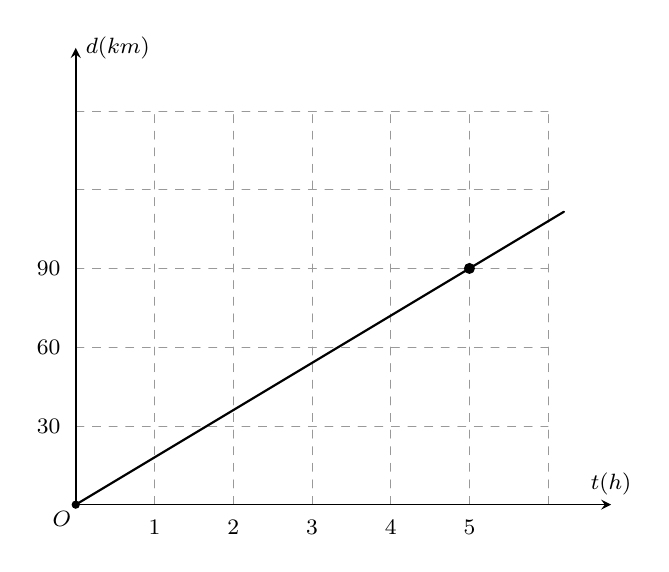
\begin{tikzpicture}[>=stealth, line join=round, line cap=round, font=\footnotesize, scale=1]
		% Định nghĩa tọa độ gốc
		\path (0,0) coordinate (O);
		% Vẽ lưới tọa độ nét đứt
		\draw[dashed, black!40, very thin] (0, 0) grid (6, 5);
		% Vẽ hai trục tọa độ
		\draw[->, semithick] (0, 0) -- (6.8, 0) node[above] {$t\text{ (h)}$};
		\draw[->, semithick] (0, 0) -- (0, 5.8) node[right] {$d\text{ (km)}$};
		% Vẽ đường thẳng đồ thị
		\draw[thick] (0, 0) -- (6.2, 3.72);
		% Đánh dấu điểm đặc biệt (5; 90) tương ứng với (5; 3) trên hệ lưới
		\fill[black] (5, 3) circle (2pt);
		% Nhãn trên các trục
		\foreach \x in {1,2,3,4,5} {
			\node[below=2pt] at (\x, 0) {$\x$};
		}
		\foreach \y/\val in {1/30, 2/60, 3/90} {
			\node[left=2pt] at (0, \y) {$\val$};
		}
		% Nhãn điểm gốc tọa độ O
		\foreach \p/\g in {O/-135}
		\fill[black] (\p) circle (1.5pt) ++(\g:0.25) node{$\p$};
	\end{tikzpicture}
\end{center}
		\shortans[]{4,2}
		\loigiai{
			\begin{itemize}
				\item Đồ thị $(d-t)$ mang hình dạng một đoạn thẳng dốc hướng lên đi qua gốc tọa độ, chứng tỏ chiếc xe ô tô thực hiện chuyển động thẳng đều.
				\item Vận tốc của xe ô tô tính theo đơn vị $\text{km/h}$: $v = \frac{d}{t} = \frac{60\text{ km}}{4\text{ h}} = 15\text{ km/h}$.
				\item Thực hiện quy đổi vạch đơn vị sang hệ mốc tiêu chuẩn mét trên giây ($\text{m/s}$):
				$$v = \frac{15}{3,6}\text{ m/s} \approx 4,166\text{ m/s} \approx 4,2\text{ m/s} \text{}$$
				*(Lưu ý đối chiếu lại vạch số nháp viết tay $18,5$ bị ghi nhầm hệ số đổi của tệp gốc).*
			\end{itemize}
		}
	\end{ex}
	
	\begin{ex}%[10V1-207-17]
		Một người lái xe máy đang cho xe vận hành chạy đều với vận tốc dải hằng số $28,8\text{ km/h}$ thì bất ngờ phát hiện nhìn thấy một cái hố sâu nguy hiểm nằm ngay trước mặt. Người lái xe kịp thời đạp phanh gấp hết cỡ, xe máy thực hiện trượt chậm dần đều thêm một khoảng thời gian dài $5\text{ s}$ nữa thì dừng lại hẳn. Tính giá trị hằng số gia tốc trung bình của xe máy thu được trong tiến trình phanh xe đó theo đơn vị $\text{m/s}^2$?
		\shortans[]{-1,6}
		\loigiai{
			\begin{itemize}
				\item Tiến hành quy đổi vận tốc xuất phát ban đầu sang đơn vị hệ mốc mét trên giây: $v_0 = 28,8\text{ km/h} = \frac{28,8}{3,6} = 8\text{ m/s}$.
				\item Khi xe máy dừng lại hẳn hoàn toàn, giá trị vận tốc cuối bằng triệt tiêu: $v = 0\text{ m/s}$.
				\item Gia tốc trung bình của quá trình phanh xe máy bằng:
				$$a = \frac{v - v_0}{\Delta t} = \frac{0 - 8}{5} = -1,6\text{ m/s}^2 \text{}$$
			\end{itemize}
		}
	\end{ex}
	
	\begin{ex}%[10V1-207-18]
		Một khối hệ vật nặng cơ học được thả cho rơi tự do từ độ cao thềm vị trí ban đầu bằng $80\text{ m}$ xuống mặt đất. Lấy gia tốc trọng trường mốc quy ước $g=10\text{ m/s}^2$. Tính khoảng thời gian rơi thẳng chuyển động của vật tính từ lúc thả cho đến khi vật vừa chạm sát mặt đất theo đơn vị giây (s)?
		\shortans[]{4}
		\loigiai{
			\begin{itemize}
				\item Hệ thức tính hành trình quãng đường rơi thẳng tự do từ trạng thái tĩnh: $h = \frac{1}{2}gt^2$.
				\item Thay các số liệu đại số vào phương trình để giải tìm biến số thời gian chạm đất $t$:
				$$80 = \frac{1}{2} \cdot 10 \cdot t^2 \Rightarrow 80 = 5t^2 \Rightarrow t^2 = 16 \Rightarrow t = 4\text{ s} \text{}$$
			\end{itemize}
		}
	\end{ex}
	
	\Closesolutionfile{ans}
	
	%%%%%%%%%%%%%%%%%%%%%%%%%%%%%%%%%%%%%%%%%%%%%%%%%%%%%%%%%%%%%%%%%%%%%%%%%
	% B. PHẦN TỰ LUẬN TỰ LUẬN BÀI TẬP (3 ĐIỂM)
	%%%%%%%%%%%%%%%%%%%%%%%%%%%%%%%%%%%%%%%%%%%%%%%%%%%%%%%%%%%%%%%%%%%%%%%%%
	\noindent \textbf{B. Phần tự luận. (3,0đ)}
	\vspace{0.2cm}
	
	\begin{ex}%[10V1-207-19]
		Vào đúng thời điểm thời gian lúc 7 giờ sáng, có một chiếc xe ô tô chuyển động thẳng đều với hằng số vận tốc tốc độ bằng $40\text{ km/h}$ di chuyển hành trình đi từ điểm A qua vạch điểm B rồi tiến tới điểm C. Biết khoảng cách đoạn đường trục đo được giữa B và A bằng $30\text{ km}$, và đoạn giữa C và B bằng $70\text{ km}$. Chọn chiều dương của hệ trục Ox hướng trùng chiều từ A đến B, gốc tọa độ tính tại điểm nút A, gốc mốc thời gian chọn lúc 7 giờ sáng. Hãy vẽ đồ thị độ dịch chuyển – thời gian $(d-t)$ mô tả hành trình của ô tô.
		\loigiai{
			\begin{itemize}
				\item Lập phương trình độ dịch chuyển của ô tô chuyển động thẳng đều từ gốc tọa độ A ($d_0 = 0$): $d(t) = v \cdot t = 40t\text{ (km)}$.
				\item Xác định tọa độ các điểm mốc chính để vẽ đồ thị:
				\begin{itemize}
					\item Tại thời điểm xuất phát lúc 7h ($t=0$): độ dịch chuyển $d = 0$ (Vị trí A).
					\item Xe đi qua điểm B cách A $30\text{ km}$ $\Rightarrow 30 = 40t_{\text{B}} \Rightarrow t_{\text{B}} = 0,75\text{ h}$ (Lúc 7h45 phút).
					\item Xe tiến tới điểm cực biên C cách A tổng cộng là $d_{\text{C}} = AB + BC = 30 + 70 = 100\text{ km}$. Thời điểm tới C: $100 = 40t_{\text{C}} \Rightarrow t_{\text{C}} = 2,5\text{ h}$ (Lúc 9h30 phút).
				\end{itemize}
				\item \textbf{Thao tác đồ thị:} Trên hệ trục tọa độ $(d-t)$ với trục đứng $d\text{ (km)}$ và trục ngang $t\text{ (h)}$, đồ thị biểu diễn là một đoạn thẳng nối liền xuất phát từ gốc tọa độ $O(0;0)$ kéo dài dốc hướng lên đi qua vạch điểm tọa độ hình học $B(0;75;30)$ và dừng lại tại điểm nút kết thúc hành trình $C(2,5;100)$.
			\end{itemize}
		}
	\end{ex}
	
	\begin{ex}%[10V1-207-20]
		Một vật thể nhỏ thực hiện chuyển động thẳng biến đổi đều dọc theo một trục tọa độ Ox có đồ thị vận tốc – thời gian $(v-t)$ được biểu diễn qua đường thẳng dốc lên như hình vẽ đính kèm bên. Trích xuất số liệu đồ thị chỉ rõ: tại mốc đầu $t=0$ thì vận tốc bằng $v_0 = 2\text{ m/s}$, và tại thời điểm sau thời gian $t = 10\text{ s}$ vận tốc đạt vạch mức $v = 12\text{ m/s}$. Hãy tính:
% TODO: \usepackage{graphicx} required
\begin{center}
	%\includegraphics[scale=1]{HINHVE-phai-Tikz/VL10-GHKI-BTX-2526-hinh3}
	\begin{tikzpicture}[>=stealth, line join=round, line cap=round, font=\footnotesize, scale=1]
		% Định nghĩa tọa độ các điểm mốc
		\path (0,0) coordinate (O);
		\path (1.5,2.0) coordinate (A);
		\path (4.5,2.0) coordinate (B);
		\path (1.5,0) coordinate (T1);
		\path (4.5,0) coordinate (T2);
		\path (0,2.0) coordinate (V1);
		% Vẽ hệ trục tọa độ
		\draw[->] (-0.5, 0) -- (6.0, 0) node[below] {$t\text{ (s)}$};
		\draw[->] (0, -0.5) -- (0, 3.0) node[right] {$v\text{ (m/s)}$};
		% Vẽ đồ thị chính (nét liền)
		\draw[thick] (O) -- (A) -- (B);
		% Vẽ các đường gióng vuông góc (nét đứt)
		\draw[dashed] (V1) -- (A) -- (T1);
		\draw[dashed] (B) -- (T2);
		% Nhãn tọa độ trên các trục
		\node[below left] at (O) {$O$};
		\node[left] at (V1) {$10$};
		\node[below] at (T1) {$10$};
		\node[below] at (T2) {$30$};
	\end{tikzpicture}
\end{center}
		\begin{enumerate}
			\item[a, ] Giá trị hằng số gia tốc $a$ của chuyển động thẳng biến đổi đều này?
			\item[b, ] Tổng quãng đường $s$ mà vật thể nhỏ đã đi được sau khoảng thời gian $10\text{ giây}$ đếm từ mốc đầu?
		\end{enumerate}
		\loigiai{
			\begin{enumerate}
				\item[a, ] Áp dụng công thức động học trích xuất tính trị số gia tốc từ biến thiên vận tốc:
				$$a = \frac{v - v_0}{t} = \frac{12 - 2}{10} = \frac{10}{10} = 1\text{ m/s}^2 \text{}$$
			\end{enumerate}
			\begin{enumerate}
				\item[b, ] Vì trong suốt khoảng thời gian $10\text{ s}$ vật luôn chuyển động thẳng dốc lên một chiều theo chiều dương ($v > 0$), nên quãng đường đi được trùng khít với độ lớn độ dịch chuyển tính theo phương trình hình học:
				$$s = v_0 t + \frac{1}{2}at^2 = 2 \cdot 10 + \frac{1}{2} \cdot 1 \cdot 10^2 = 20 + 50 = 70\text{ m} \text{}$$
			\end{enumerate}
		}
	\end{ex}
	
	\begin{ex}%[10V1-207-21]
		Người ta thực hiện thao tác thả rơi tự do cho một hệ vật nặng chuyển động đổ xuống từ độ cao vị trí ban đầu bằng $100\text{ m}$ thẳng hướng xuống mặt đất. Lấy gia tốc trọng trường mốc quy ước $g=10\text{ m/s}^2$. Hãy xác định:
		\begin{enumerate}
			\item[a, ] Tổng hành trình quãng đường vật nặng rơi dời chỗ được sau khoảng thời gian $3\text{ s}$ tính từ lúc thả?
			\item[b, ] Độ cao thực tế của vật nặng so với mặt đất tại thời điểm sau khi thả rơi được $3\text{ s}$?
		\end{enumerate}
		\loigiai{
			\begin{enumerate}
				\item[a, ] Áp dụng phương trình công thức tính quãng đường rơi tự do của hệ vật tại thời điểm $t=3\text{ s}$:
				$$s(3) = \frac{1}{2}gt^2 = \frac{1}{2} \cdot 10 \cdot 3^2 = 5 \cdot 9 = 45\text{ m} \text{}$$
			\end{enumerate}
			\begin{enumerate}
				\item[b, ] Độ cao thực tế của vật nặng so với vạch mốc mặt đất bằng hiệu số giữa độ cao ban đầu và khoảng quãng đường vật đã đổ rơi xuống được:
				$$h' = h - s(3) = 100\text{ m} - 45\text{ m} = 55\text{ m} \text{}$$
			\end{enumerate}
		}
	\end{ex}
	
	\Closesolutionfile{ans}
	
	\newpage
	%%%%%%%%%%%%%%%%%%%%%%%%%%%%%%%%%%%%%%%%%%%%%%%%%%%%%%%%%%%%%%%%%%%%%%%%%
	% KHUNG ĐÁP ÁN BẢNG TỰ ĐỘNG IN KẾT XUẤT CỦA HỆ THỐNG
	%%%%%%%%%%%%%%%%%%%%%%%%%%%%%%%%%%%%%%%%%%%%%%%%%%%%%%%%%%%%%%%%%%%%%%%%%
	\begin{center} \textbf{BẢNG ĐÁP ÁN THAM KHẢO LỚP 10 --- MÃ ĐỀ 207} \end{center}
	
	\noindent \textbf{Phần I (Câu hỏi trắc nghiệm nhiều phương án lựa chọn):}  
	\indapan{12}{ans/ansTN-BuiThiXuan207}
	
	\noindent \textbf{Phần II (Câu hỏi trắc nghiệm Đúng/Sai):}
	\indapan[TF]{2}{ans/ansTF-BuiThiXuan207}
	
	\noindent \textbf{Phần III (Câu hỏi trắc nghiệm trả lời ngắn):}
	\indapan[SA]{4}{ans/ansSA-BuiThiXuan207}
	
	\label{B\thedeso}
	